%==============================================================
%  CS-C3240 Machine Learning
%  Project: Predicting Finland's electricity consumption
%           from the weather and time
%  Compile:  latexmk -pdf report.tex     (or pdflatex + bibtex + pdflatex x2)
%==============================================================
\documentclass[11pt,a4paper]{article}

%---------------- Fill these in -------------------------------
\newcommand{\ReportTitle}{Predicting Finland's electricity consumption from the weather and time}
%--------------------------------------------------------------

\usepackage[utf8]{inputenc}
\usepackage[T1]{fontenc}
\usepackage[english]{babel}
\usepackage{lmodern}
\usepackage[margin=2.5cm,headheight=14pt,includehead]{geometry}
\usepackage{graphicx}
\usepackage{booktabs}
\usepackage{enumitem}
\usepackage{xcolor}
\usepackage{caption}
\usepackage{subcaption}
\usepackage{float}
\usepackage{fancyhdr}
\usepackage{amsmath}
\usepackage{amssymb}
\usepackage{textcomp}
\usepackage[numbers]{natbib}
\usepackage{xurl}
\usepackage[hidelinks]{hyperref}

% Plots are read straight from the repository's eda_plots folder
\graphicspath{{../eda_plots/}{figures/}}
% Let tall figures share a page with text instead of getting a page of their own
\renewcommand{\topfraction}{0.9}
\renewcommand{\bottomfraction}{0.6}
\renewcommand{\textfraction}{0.08}
\renewcommand{\floatpagefraction}{0.8}

\setlength{\parskip}{0.6em}
\setlength{\parindent}{0pt}

\pagestyle{fancy}
\fancyhf{}
\lhead{CS-C3240 Machine Learning}
\rhead{Project report}
\cfoot{\thepage}

% Grey guidance note -- delete these once you have written the section
\newcommand{\guide}[1]{{\small\itshape\color{gray}(#1)}}
% Feature / column names in typewriter font, e.g. \feat{temp_c}
\newcommand{\feat}[1]{\texttt{\detokenize{#1}}}

\begin{document}

%---------------- Title block ---------------------------------
\begin{center}
  {\large\bfseries CS-C3240 Machine Learning}\\[0.4em]
  {\large\bfseries \ReportTitle}\\[0.4em]
  {\large Project report}\\[0.4em]
  {\today}
\end{center}

%==============================================================
\section{Introduction}

Weather affects how people use electricity. Cold weather increases demand for heating,
while hot weather causes air conditioners to run longer. Strong winds draw heat away
from structures more quickly, further increasing heating demand. High humidity makes
buildings feel hotter than they actually are, increasing demand for air conditioning. Low
humidity, on the other hand, makes buildings feel colder, increasing demand for
heating~\cite{montel2024weather}. Electricity consumption also follows daily and weekly
patterns independent of weather, since usage tends to vary by hour of the day and by day
of the week~\cite{eia2011demand}.

The goal of this project is to predict how weather conditions in Finland, namely
temperature, wind, and humidity, along with the hour of day, weekday and month, affect
electricity consumption. This is done by combining data from Fingrid, the Finnish
electricity transmission system operator, and the Finnish Meteorological Institute (FMI).
This report consists of an introduction, problem formulation, methods, results,
conclusion, and references. The methods section further consists of data preparation,
model choice and model validation.

%==============================================================
\section{Problem formulation}

The data in this study comes from Fingrid and the Finnish Meteorological Institute (FMI).
The electricity data is the ``Electricity consumption in Finland'' dataset from Fingrid's open
data service~\cite{fingrid2026consumption}, comprising 119\,369 measurements, and the weather
data consists of 52\,589 hourly observations from the FMI Tapiola weather station, downloaded
from FMI's open data service~\cite{fmi2026observations}. Both cover the years 2020--2025.

Each data point represents one hour and has seven numerical features: air temperature
in degrees Celsius (\feat{temp_c}), wind speed in metres per second (\feat{wind_ms}), relative
humidity as a percentage (\feat{humid_pc}), a cyclic encoding of the hour of day as sine and
cosine (\feat{hour_sin}, \feat{hour_cos}), the weekday as an integer from 1 to 7 (\feat{weekday}),
and the month as an integer from 1 to 12 (\feat{month}). The hour of day is encoded cyclically
so that hour 23 and hour 0 are treated as adjacent rather than maximally distant. The label is
the average electricity consumption in Finland during that hour, measured in
megawatt-hours (\feat{consumption_mwh}). Since the label is continuous, this is a supervised
regression problem. The first rows of the merged data are shown in Table~\ref{tab:raw-data}.

\begin{table}[H]
  \centering
  \scriptsize
  \setlength{\tabcolsep}{3pt}
  \resizebox{\textwidth}{!}{%
  \begin{tabular}{llrrrrrrrrrr}
    \toprule
    \feat{time_utc} & \feat{local_time} & \feat{consumption_mwh} & \feat{temp_c} & \feat{wind_ms} &
    \feat{humid_pc} & \feat{hour} & \feat{hour_sin} & \feat{hour_cos} & \feat{weekday} &
    \feat{is_weekend} & \feat{month} \\
    \midrule
    2019-12-31T22:00:00Z & 2020-01-01 00:00:00 & 9822 & $-1.5$ & 4.3 & 83 & 0 & 0.0000 & 1.0000 & 3 & 0 & 1 \\
    2019-12-31T23:00:00Z & 2020-01-01 01:00:00 & 9548 & $-1.1$ & 4.3 & 85 & 1 & 0.2588 & 0.9659 & 3 & 0 & 1 \\
    2020-01-01T01:00:00Z & 2020-01-01 03:00:00 & 9141 & $-0.7$ & 4.5 & 87 & 3 & 0.7071 & 0.7071 & 3 & 0 & 1 \\
    2020-01-01T02:00:00Z & 2020-01-01 04:00:00 & 9149 & 0.1    & 5.4 & 83 & 4 & 0.8660 & 0.5000 & 3 & 0 & 1 \\
    2020-01-01T03:00:00Z & 2020-01-01 05:00:00 & 9206 & 0.5    & 5.2 & 82 & 5 & 0.9659 & 0.2588 & 3 & 0 & 1 \\
    2020-01-01T04:00:00Z & 2020-01-01 06:00:00 & 9432 & 0.3    & 4.7 & 83 & 6 & 1.0000 & 0.0000 & 3 & 0 & 1 \\
    2020-01-01T05:00:00Z & 2020-01-01 07:00:00 & 9419 & 0.1    & 4.7 & 85 & 7 & 0.9659 & $-0.2588$ & 3 & 0 & 1 \\
    2020-01-01T06:00:00Z & 2020-01-01 08:00:00 & 9558 & 0.8    & 4.9 & 81 & 8 & 0.8660 & $-0.5000$ & 3 & 0 & 1 \\
    2020-01-01T07:00:00Z & 2020-01-01 09:00:00 & 9522 & 1.5    & 4.6 & 77 & 9 & 0.7071 & $-0.7071$ & 3 & 0 & 1 \\
    \bottomrule
  \end{tabular}}
  \caption{The first rows of the merged raw data (\feat{hour_sin} and \feat{hour_cos} rounded to four decimals).}
  \label{tab:raw-data}
\end{table}

%==============================================================
\section{Methods}

\subsection{Preparing the data}

The dataset is composed of 52\,241 data points. It is merged from two datasets:
Fingrid's national electricity consumption data and FMI's weather data.
Fingrid reported consumption hourly before 13 June 2023 and every 15 minutes
thereafter, so the Fingrid data was first aggregated to hourly resolution by averaging all
measurements within each hour. The two datasets were then merged on the hourly
timestamp. 250 hours were discarded because they lacked temperature, wind speed or
humidity observations, which gives the final 52\,241 data points.

We selected temperature, wind, and humidity based on known physical effects on
heating and cooling demand, and included hour of day, weekday, and month to capture
daily and seasonal consumption patterns. We decided to drop the columns \feat{time_utc},
\feat{local_time}, \feat{hour}, and \feat{is_weekend}. Columns \feat{time_utc}, \feat{local_time},
and \feat{hour} are redundant once cyclically encoded as \feat{hour_sin} and \feat{hour_cos}, and
raw timestamp values are not directly usable as model features. Column \feat{is_weekend} is
redundant given that \feat{weekday} already captures the same information.
Figures~\ref{fig:temp}--\ref{fig:humid} show how consumption varies with each of the
selected features.

\begin{figure}[H]
  \centering
  \captionsetup{justification=raggedright,singlelinecheck=false}
  \begin{minipage}[t]{0.31\textwidth}
    \centering
    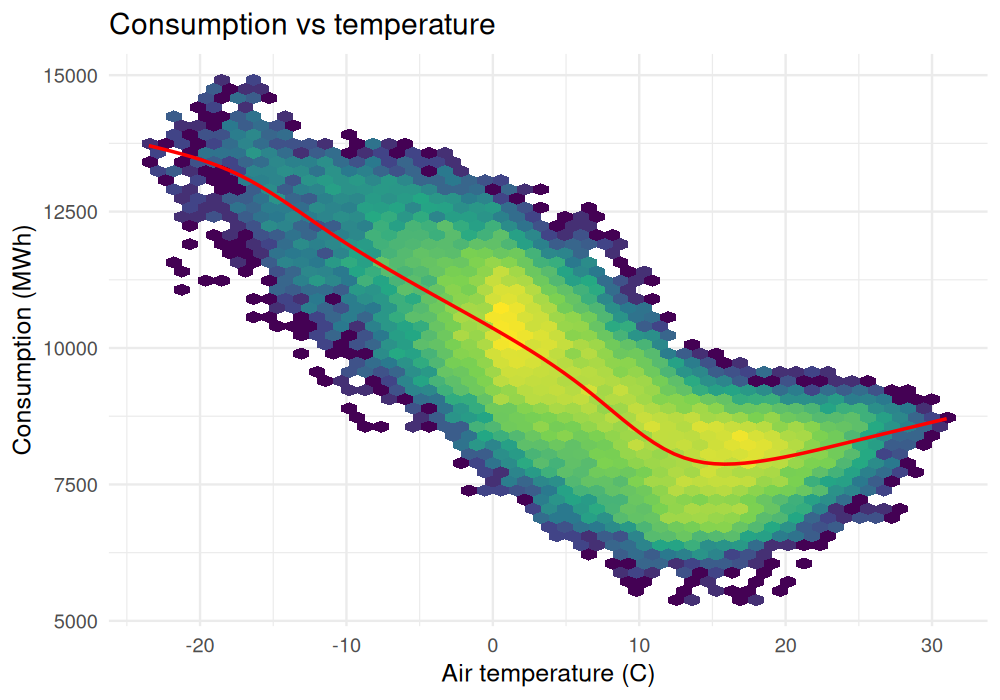
\includegraphics[width=\textwidth]{01_consumption_vs_temperature.png}
    \caption{Consumption against air temperature.}
    \label{fig:temp}
  \end{minipage}\hfill
  \begin{minipage}[t]{0.31\textwidth}
    \centering
    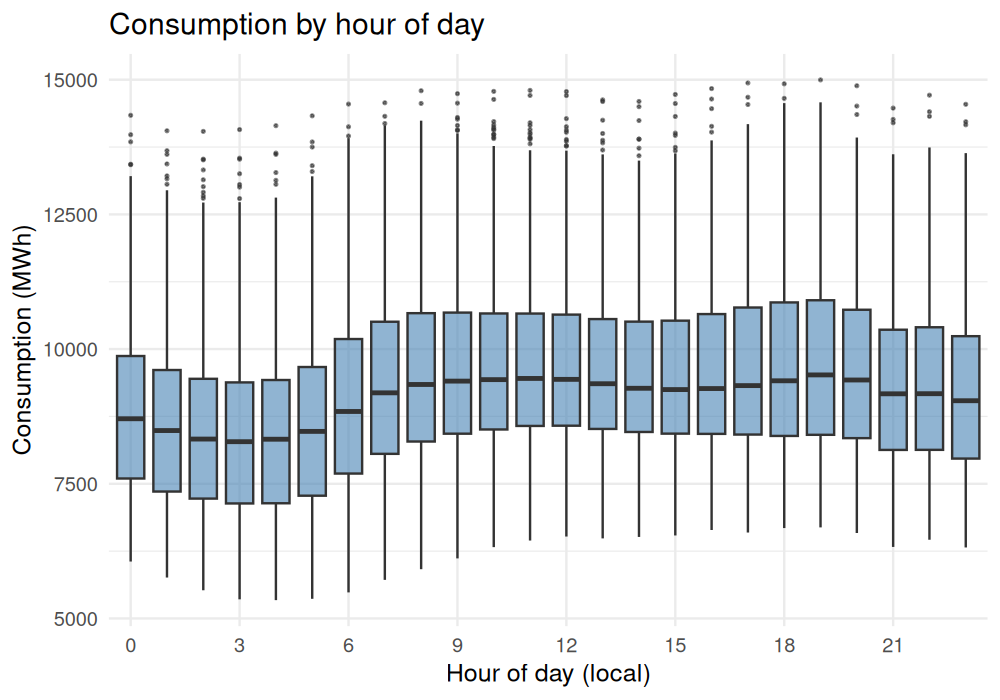
\includegraphics[width=\textwidth]{02_consumption_by_hour.png}
    \caption{Consumption by hour of day.}
    \label{fig:hour}
  \end{minipage}\hfill
  \begin{minipage}[t]{0.31\textwidth}
    \centering
    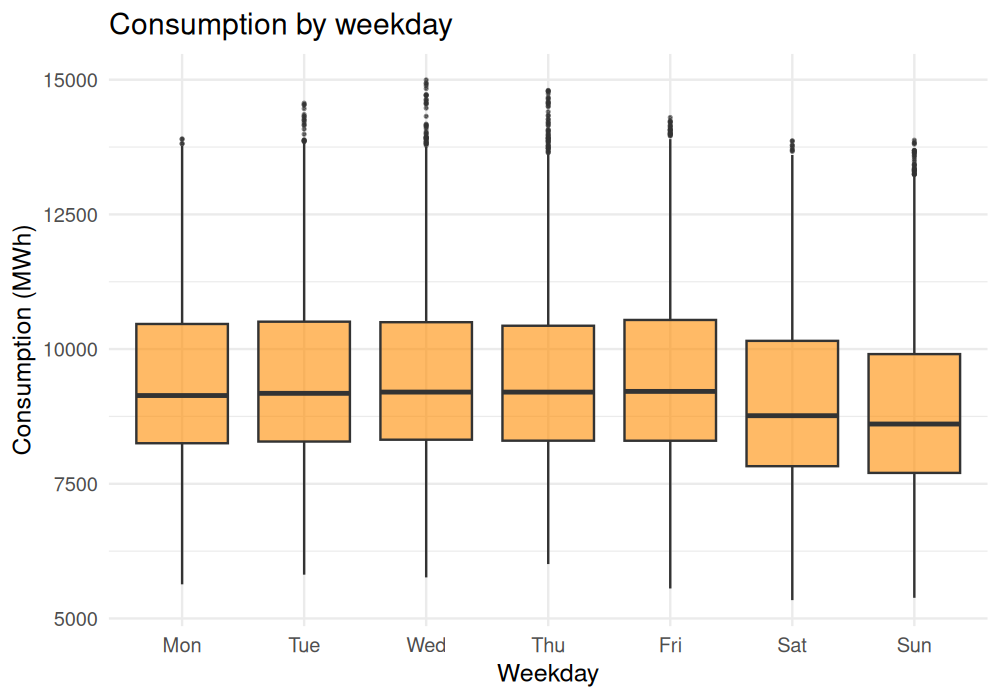
\includegraphics[width=\textwidth]{03_consumption_by_weekday.png}
    \caption{Consumption by weekday.}
    \label{fig:weekday}
  \end{minipage}

  \vspace{1em}

  \begin{minipage}[t]{0.31\textwidth}
    \centering
    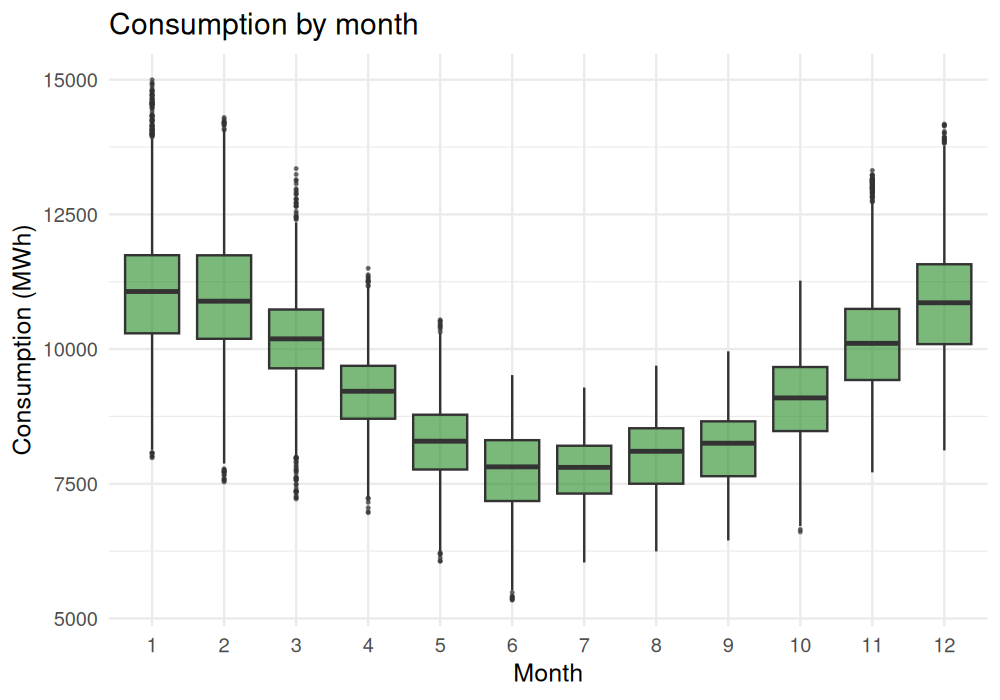
\includegraphics[width=\textwidth]{04_consumption_by_month.png}
    \caption{Consumption by month.}
    \label{fig:month}
  \end{minipage}\hfill
  \begin{minipage}[t]{0.31\textwidth}
    \centering
    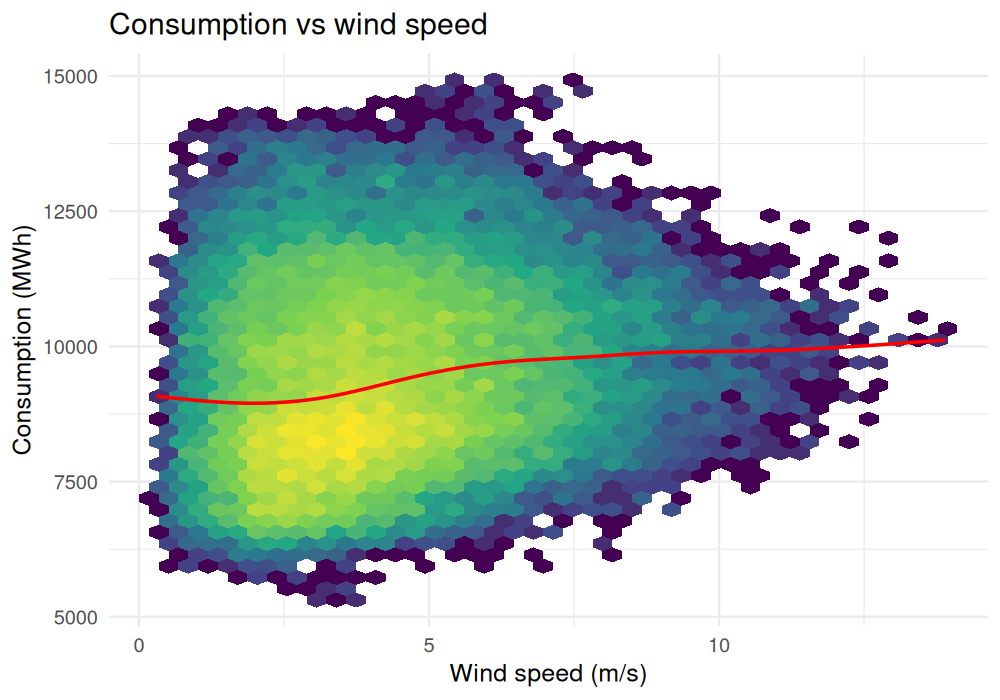
\includegraphics[width=\textwidth]{05_consumption_vs_wind_speed.png}
    \caption{Consumption against wind speed.}
    \label{fig:wind}
  \end{minipage}\hfill
  \begin{minipage}[t]{0.31\textwidth}
    \centering
    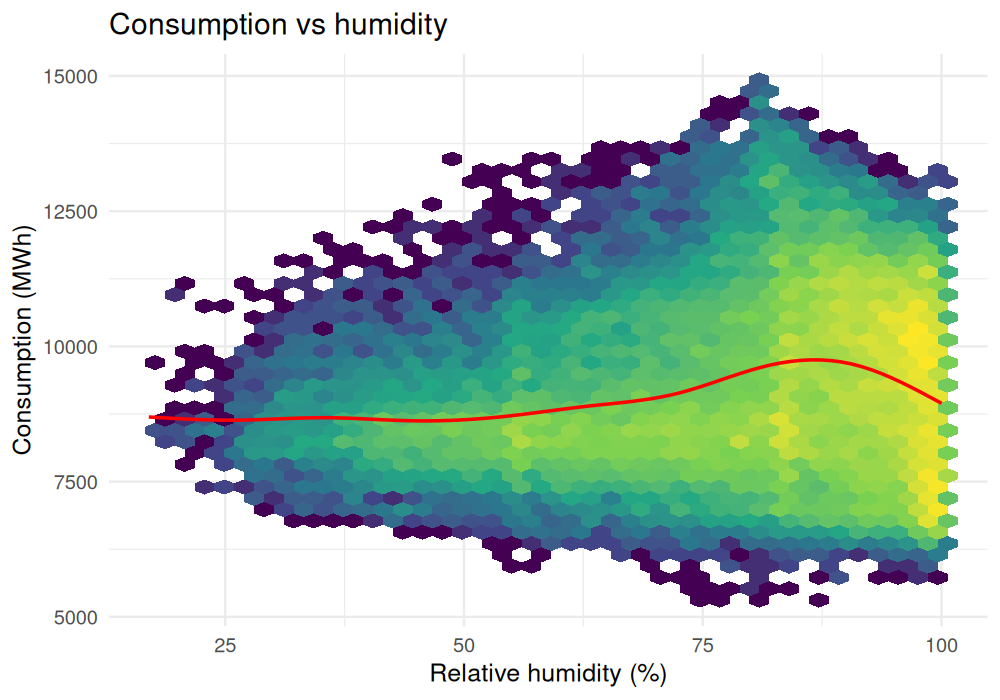
\includegraphics[width=\textwidth]{06_consumption_vs_humidity.png}
    \caption{Consumption against relative humidity.}
    \label{fig:humid}
  \end{minipage}
\end{figure}

Weekday and month were kept as plain integers rather than cyclically encoded.
Unlike hour, where the wraparound between 23:00 and 00:00 occurs within a single day
and directly affects short-term consumption patterns, the wraparound effects for
weekday and month are less pronounced for this application. The date is only used after
processing to sort the input data chronologically for comparison.

\subsection{Model}

We decided to use a linear regression model for this project, with a hypothesis space
consisting of all linear functions of the input features \feat{temp_c}, \feat{wind_ms},
\feat{humid_pc}, \feat{hour_sin}, \feat{hour_cos}, \feat{weekday}, and \feat{month}, together
with the squared temperature (see below). This decision
was made because the label we are trying to predict is continuous. Linear regression is also a
simple baseline that trains instantly on 52\,000 rows, and its coefficients are directly
interpretable.

Since our dataset consists of data points with numeric labels, this is a regression
problem, and we chose squared error loss as our loss function. Squared error loss
penalizes large prediction errors much more than small ones. This is useful for our
problem because large errors in predicted electricity consumption could cause grid
operators to over- or under-supply electricity, which is more costly than a small prediction
error.

The correlation matrix (Figure~\ref{fig:corr}) shows a strong linear relationship between
temperature and consumption ($r = -0.77$), which supports the use of linear predictors. The
scatter plot in Figure~\ref{fig:temp} nevertheless shows that this relationship flattens above
approximately 15\,\textdegree C, so a squared temperature term was added to the hypothesis
space. The predictor remains linear in its parameters and is therefore still a linear
regression model:
\begin{equation}
  \begin{split}
  h(\mathbf{x}) = {} & w_0 + w_1 x_{\text{temp}} + w_2 x_{\text{temp}}^2 + w_3 x_{\text{wind}}
  + w_4 x_{\text{humid}} \\
  & + w_5 x_{\text{hour\_sin}} + w_6 x_{\text{hour\_cos}}
  + w_7 x_{\text{weekday}} + w_8 x_{\text{month}}.
  \end{split}
  \label{eq:hypothesis}
\end{equation}

The weights are learned by minimising the squared error loss
\begin{equation}
  L\bigl((\mathbf{x}, y), h\bigr) = \bigl( y - h(\mathbf{x}) \bigr)^2,
  \label{eq:loss}
\end{equation}
where $y$ is the measured consumption and $h(\mathbf{x})$ the predicted consumption
of a data point.

\begin{figure}[htbp]
  \centering
  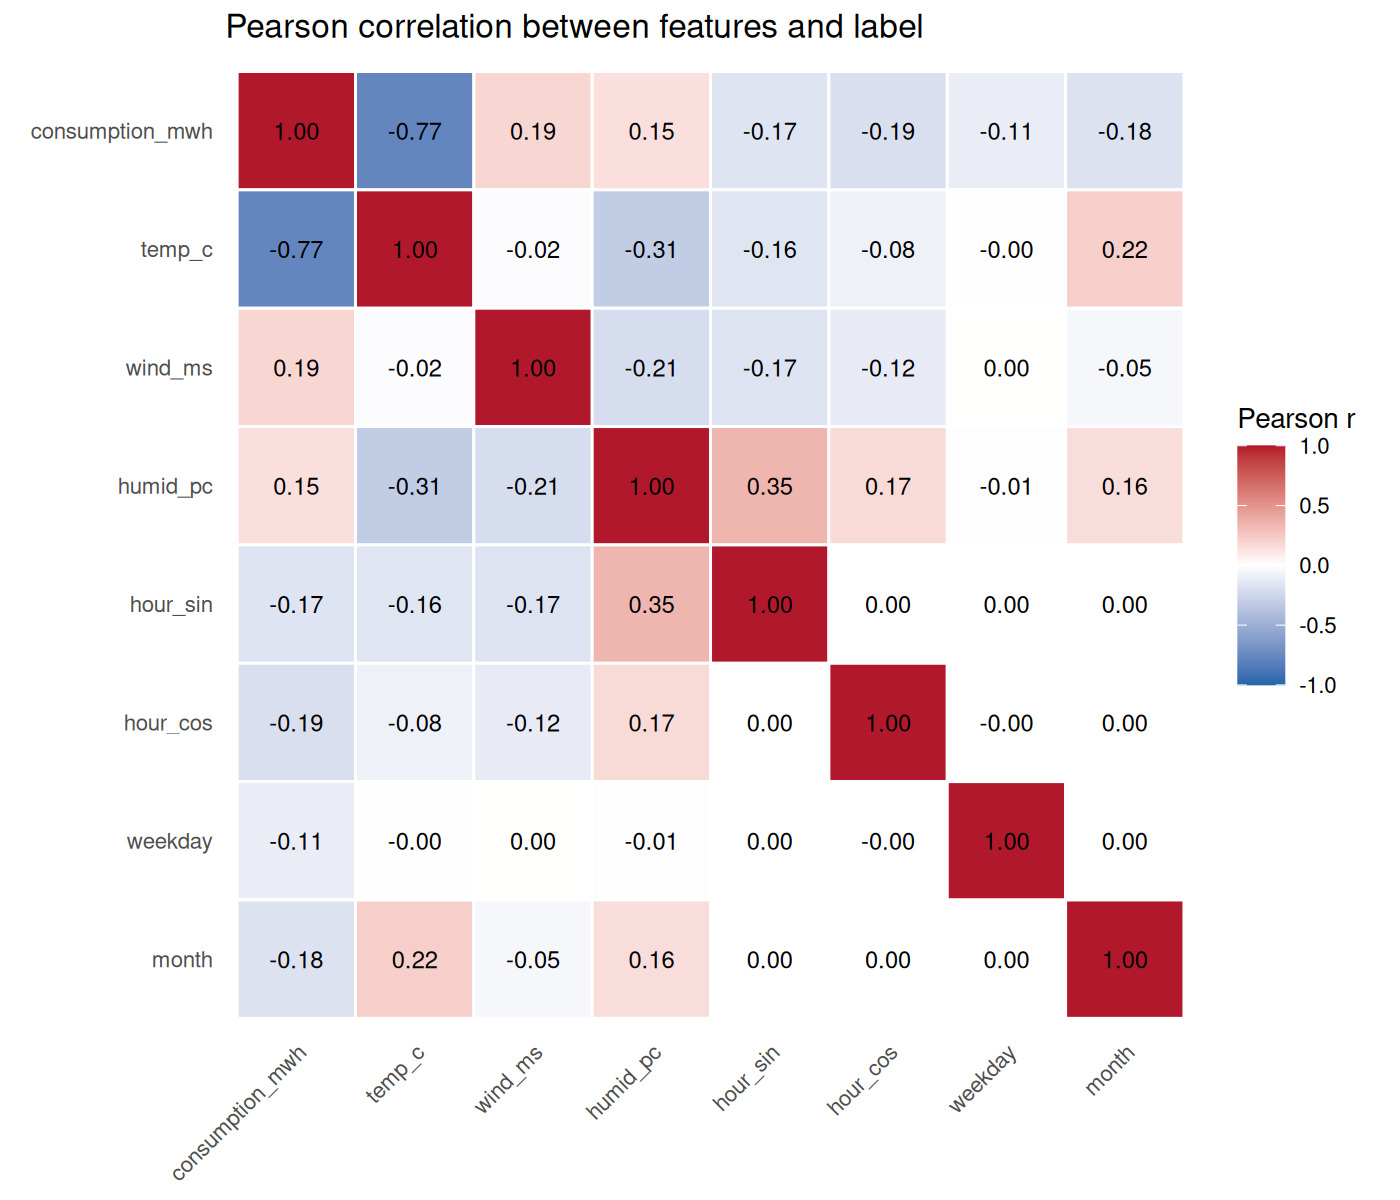
\includegraphics[width=0.6\textwidth]{correlation_matrix.png}
  \caption{Pearson correlation matrix of the features and the label.}
  \label{fig:corr}
\end{figure}

\subsection{Model validation}

For model validation the dataset was split chronologically by calendar year. The years
2020--2023 were used for training (34\,717 data points, 66.5\%), 2024 for validation
(8\,778 data points, 16.8\%) and 2025 for testing (8\,746 data points, 16.7\%).

We chose this chronological split instead of a random one as we intend to use the model to
predict future consumption based on the weather and time data. Thus the validation and test
sets must represent time periods the model has not seen during training. Second, consumption
in consecutive hours is highly correlated, so a random split would place nearly identical data
points in both the training and validation sets. Thus it could give an over-optimistic estimate
of its performance when the model interpolates between hours.

Splitting on whole calendar years also ensures that each set covers a complete annual cycle.
Had the split been made at an arbitrary point in time, the test set might have contained only
summer or only winter months, and the reported error would have reflected a single season
rather than year-round performance.

%==============================================================
\section{Use of AI}

We used AI to help write the R scripts to draw the plots. AI was also used to fix grammar and format the LaTeX document.

%==============================================================
%  References -- entries live in references.bib and are numbered
%  in the order they are first cited (\bibliographystyle{unsrtnat}).
\bibliographystyle{unsrtnat}
\bibliography{references}

%==============================================================
\appendix
\section*{Appendix}

Code: \url{https://github.com/Erkkuleo/ML-project-predicting-consumption-from-weather}

\end{document}
